\documentclass[article]
\usepackage{tikz}

\begin{document}
\title{Shapes}

\maketitle
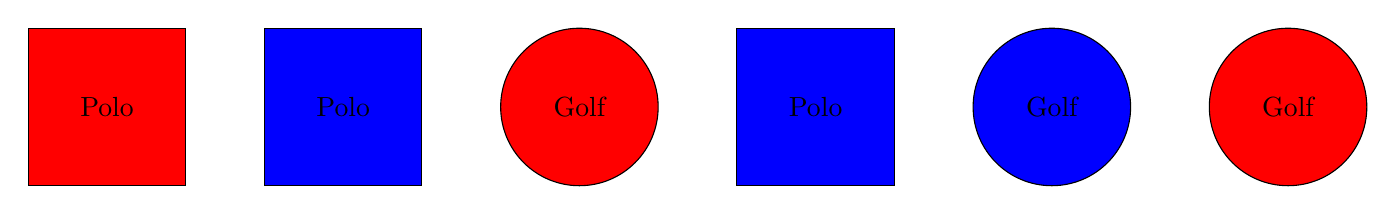
\begin{tikzpicture}

\node[rectangle, draw, fill=red!100, minimum width = 2cm, 
minimum height = 2 cm] (r) at (-1, 1) {Polo};
\node[rectangle, draw, fill=blue!100, minimum width = 2cm, 
minimum height = 2 cm] (r) at (2, 1) {Polo};
\node[circle, draw, fill=red!100, minimum width = 2cm, 
minimum height = 2 cm] (c) at (5, 1) {Golf};
\node[rectangle, draw, fill=blue!100, minimum width = 2cm, 
minimum height = 2 cm] (r) at (8, 1) {Polo};
\node[circle, draw, fill=blue!100, minimum width = 2cm, 
minimum height = 2 cm] (c) at (11, 1) {Golf};
\node[circle, draw, fill=red!100, minimum width = 2cm, 
minimum height = 2 cm] (c) at (14, 1) {Golf};

\end{tikzpicture}

\end{document}
